\documentclass[11pt,a4paper]{article}
\usepackage[utf8]{inputenc}
\usepackage[T1]{fontenc}
\usepackage{amsfonts}
\usepackage[french]{babel}
\frenchbsetup{StandardLists=true} % à inclure si on utilise \usepackage[francais]{babel}
\usepackage{enumitem}
\usepackage{amssymb}
\usepackage{amsmath}
\usepackage[left=2cm,right=2cm,top=2cm,bottom=2cm]{geometry}
\usepackage{multirow}
\usepackage[dvipsnames]{xcolor}

\usepackage[T1]{fontenc}
\usepackage{fouriernc}
\usepackage{graphicx}
\usepackage{colortbl}

\usepackage{setspace}
\singlespacing

\usepackage{pstricks}
\usepackage{xkeyval}
\usepackage{pst-labo}


\usepackage{multicol}
\usepackage{caption}
\usepackage{fancyhdr}
\pagestyle{fancy}
\renewcommand\headrulewidth{1pt}
\fancyhead[L]{Lycée Denis Diderot }
\fancyhead[R]{Classe de 1 Bac Pro }
\setcounter{page}{5}\fancyfoot[C]{page \thepage}
\fancyfoot[R]{Année 2024-2025}
\fancyfoot[L]{Alexis RUIZ}
\usepackage{multirow,tabularx,booktabs}
\newcommand{\cadreblanc}[1]{%
\medskip\framebox[\linewidth][c]{%
\rule{0mm}{#1mm}}\par
\medskip}

\usepackage{awesomebox}
\setlength{\aweboxvskip}{0mm}
\usepackage{pifont}
\usepackage{chemmacros}
\chemsetup{modules=all}
\setlength{\columnseprule}{.25mm}

\renewcommand{\arraystretch}{2}
\newcolumntype{C}[1]{>{\centering\arraybackslash }b{#1}}

\newcommand*\acocher{\quitvmode{\fboxsep0pt \fboxrule0.8pt \fbox{\vrule height1.8ex depth.1ex width0pt \vrule height0pt depth0pt width1.9ex }}}

\newcommand{\code}{\awesomebox[black]{2pt}{

\includegraphics[scale=0.15]{../Chapitre 1 - Energie et puissance électrique/images/frame.png}
}{black}}

\newcommand{\moteur}{\awesomebox[black]{2pt}{

\includegraphics[scale=1]{images/moteur.jpg} 
}{black}}

\newcommand{\defconclusion}{\awesomebox[black]{2pt}{\rotatebox{90}{\Large{\textbf{Conclusion}}}}{black}}


  \newenvironment{itemize*}%  % listes compactes
    {\begin{itemize}%
      \setlength{\itemsep}{0pt}%
      \setlength{\parskip}{0pt}}%
    {\end{itemize}}


\frenchbsetup{StandardLists=true}
\newlist{fleche}{itemize}{1}
\setlist[fleche]{label=\ding{220},font=\color{orange}}





\begin{document}


\begin{center}
 \LARGE{COURS } \\[3mm]
\end{center}



\normalsize

\hrule\
\\[0,5cm]


\fcolorbox{black}{white}{\textbf{\ding{202} Puissance dissipée par effet Joule. }}\\
\vspace{-3mm}
\begin{itemize*}
\item Cas général



\noindent%
\begin{minipage}{.65\textwidth}%
 \cadreblanc{25}
\end{minipage}%
\hfill
\begin{minipage}{.27\textwidth}%
\cadreblanc{25}
\end{minipage}%


\item Cas d'un conducteur ohmique \\
\vspace{-5mm}
\noindent%
\begin{fleche}
\item 
\begin{minipage}{.60\textwidth}%
 \cadreblanc{25}
\end{minipage}%
\hfill
\begin{minipage}{.27\textwidth}%
\cadreblanc{25}
\end{minipage}%


\noindent%
\item 
\begin{minipage}{.60\textwidth}%
 \cadreblanc{25}
\end{minipage}%
\hfill
\begin{minipage}{.27\textwidth}%
\cadreblanc{25}
\end{minipage}%
\end{fleche}

\fcolorbox{black}{white}{\textbf{\ding{203} Transformateur}}\\
\vspace{-3mm}
\noindent%
\begin{minipage}{.58\textwidth}%
\item Un transformateur est constitué d'un circuit magnétique fermé sur lequel sont enroulées deux bobines électriquement indépendantes : le \textbf{primaire}, constitué de \textbf{$\mathrm{N_1}$ }spires et le \textbf{secondaire} constitué de \textbf{$\mathrm{N_2}$} spires \\
\textcolor{red}{Remarque :} un transformateur ne fonctionne pas en régime continu.


\end{minipage}%
\hfill
\begin{minipage}{.30\textwidth}%
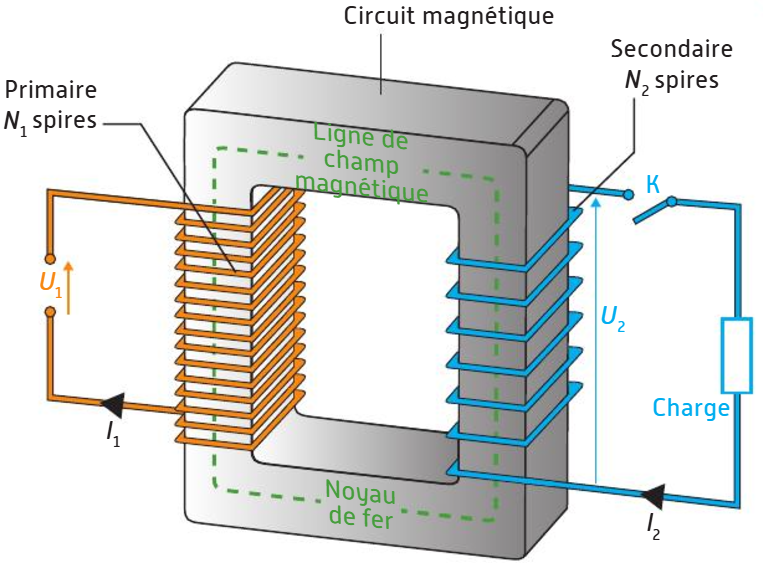
\includegraphics[width=\textwidth]{images/transformateur.png}
\end{minipage}%

\item Le \textbf{rapport de transformation \textit{m}} est défini par : 

\noindent%

\begin{minipage}{.27\textwidth}%
 \cadreblanc{18}
\end{minipage}%
\hfill
\begin{minipage}{.65\textwidth}%
\cadreblanc{18}
\end{minipage}%


\begin{minipage}{.65\textwidth}%
\item Un transformateur dans lequel les pertes sont négligeables est dit "parfait" et son rapport de transformation s'exprime ainsi : 

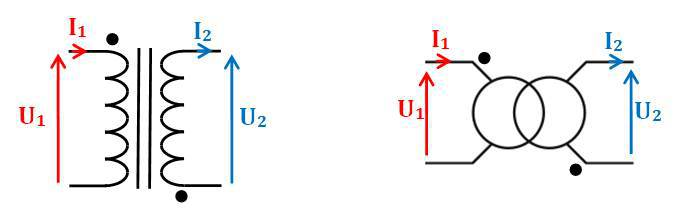
\includegraphics[scale=0.56]{images/Transfo_symboles.jpg}
\end{minipage}%
\hfill
\begin{minipage}{.27\textwidth}%
\cadreblanc{25}
\end{minipage}%

\end{itemize*}











\end{document}